\documentclass{article}

\usepackage{style}

\usepackage[utf8]{inputenc} % allow utf-8 input
\usepackage[T1]{fontenc}    % use 8-bit T1 fonts
\usepackage{hyperref}       % hyperlinks
\usepackage{url}            % simple URL typesetting
\usepackage{booktabs}       % professional-quality tables
\usepackage{amsfonts}       % blackboard math symbols
\usepackage{nicefrac}       % compact symbols for 1/2, etc.
\usepackage{microtype}      % microtypography
\usepackage{lipsum}
\usepackage{fancyhdr}       % header
\usepackage{graphicx}       % graphics
\usepackage{multicol}       % multicolumn
\usepackage{float}
\graphicspath{{media/}}     % organize your images and other figures under media/ folder

%Header
\pagestyle{fancy}
\thispagestyle{empty}
\rhead{ \textit{ }} 

% Update your Headers here
\fancyhead[LO]{SpongeDetect: An Adventure}
% \fancyhead[RE]{Firstauthor and Secondauthor} % Firstauthor et al. if more than 2 - must use \documentclass[twoside]{article}


%% Title
\title{SpongeDetect
%%%% Cite as
%%%% Update your official citation here when published 
\thanks{\textit{\underline{Citation}}: 
\textbf{Adam Hearn, Blake Bryan. SpongeDetect. Pages.... DOI:69420/8008135.}} 
}

\author{
  Adam Hearn, Blake Bryan \\
  Computer Science \\
  George Fox University \\
  Newberg\\
  \texttt{\{ahearn19, bbryan19\} @georgefox.edu} \\
}


\begin{document}
\maketitle


\begin{abstract}
% \lipsum[1]
{The following paper displays the utilization of a convolutional neural network using TensorFlow and Keras in order to detect and classify distinct Spongebob character images. Through manual data collection of the first few seasons of Spongebob combined with the proper convolutional layers and a neural network, weights and biases are derived in order to process an image and predict the output for that image. The following layers comprise the neural network in which the images are processed - Input layer, convolutional layer, pooling layer, dense layer. The CNN is used to classify images of four different Spongebob characters - Spongebob, Patrick, Squidward, and Mr Krabs.}
\end{abstract}
\vskip 0.3in


% keywords can be removed
\keywords{Convolutional Neural Networks \and Spongebob \and TensorFlow}
\vskip 0.2in
\begin{multicols}{2}

\section{Introduction}
% \lipsum[1]
% \lipsum[3]
{\quad
Nearly 23 years ago Stephen Hillenburg created the world's greatest cartoon - Spongebob Squarepants. As time has passed, Spongebob has engrained himself in pop culture earning himself all the fame he deserves. However, in recent years after the passing of the original creator, the Spongebob franchise has slowly faded into the depths of its final stretch as a children's cartoon. This disappointing turn in its existence has left the show at the beginning of its end where its content will soon become a mere memory in the minds of the aging Generation Z. As the show dissipates into its demise it is up to the research in this paper to keep the legacy alive. An extremely accurate and sought after method is required to aid those who will soon aimlessly wander the earth not knowing which Spongebob character is which. This research paper leans into utilizing a convolutional neural network that detects specific Spongebob characters in images in an attempt to fix these intense world issues. 
\newline
\quad To implement the convolutional neural network, the Tensorflow library was used alongside Keras. TensorFlow offers multiple levels of abstraction allowing for ease of use in model building. Keras is a deep learning API that runs on top of TensorFlow that is a simple, flexible, and powerful tool providing those essential abstractions for developing machine learning solutions \cite{team_keras_nodate}. See the specific implementation and explanation of our model using TensorFlow and Keras in section \ref{sec:model}. These powerful high level tools allow for this project to come alive and give a true purpose to what it means to know Spongebob characters. It is through the powers of machine learning that Spongebob's legacy shall live on.
}
\vskip 0.2in

\section{Methods}
\label{sec:headings}

% \lipsum[4] 
{\quad
The task is to accurately identify and classify images of certain Spongebob characters given the dataset of character images. By properly building and training a machine learning model, this goal can be achieved.
The initial design of the model utilized feature extraction involving the edges of objects within Spongebob frames, as well as dominant colors in the image. Both conventional SVM type models and neural networks using these features did not result in an adequate performance. After multiple trials and errors it was determined that the method of the initial design was lacking and needed to be reworked. The method of manual image feature extraction combined with the SVM classifier was trashed. \newline
\quad 
Through intense research and sheer willpower a convolutional neural network was then written. The revamped design uses Tensorflow's Keras to demonstrate image classification. With just a single layered CNN, this method saw much more success in it's ability to accurately classify Spongebob character's based off of the given image. Adding a few more layers and taking advantage of KerasTuner to tune the model's architecture further improved the model's accuracy. See Section \ref{sec:tuner} for more on the utilization of KerasTuner.
}

\subsection{Data Preparation}
% \lipsum[5]
{\quad
To prepare the data the entire, Spongebob seasons two, three, and four were downloaded.
Using FFmpeg, a FOSS video conversion utility, frames were captured every 2 seconds from each of the episodes.
From there the frames were cropped and resized to 256x256 images. See figure \ref{fig:crop}
In order to ensure a high quality data corpus was created, the images were manually selected for their respective characters and were placed in the proper character folder.
Each image that was selected is ensured to include its respective character and that character only and at a minimum contains the character's entire head in the frame.
Images were often excluded on the basis of more than one character in frame.
In addition, if the characters were visualized in a frame in a way that completely changed their appearance, this frame would be excluded.
The images being classified by the model consist of the following four characters - Spongebob, Patrick, Squidward, and Mr Krabs see Figure \ref{fig:collage}.
\vskip 0.1in
\begin{figure}[H]
  \begin{center}
    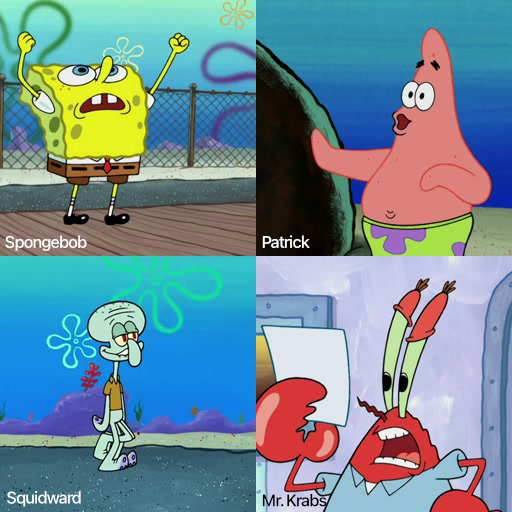
\includegraphics[width=5cm]{collage.png}
  \end{center}
  \caption{The four characters chosen to identify}
  \label{fig:collage}
\end{figure}

\begin{figure}[H]

  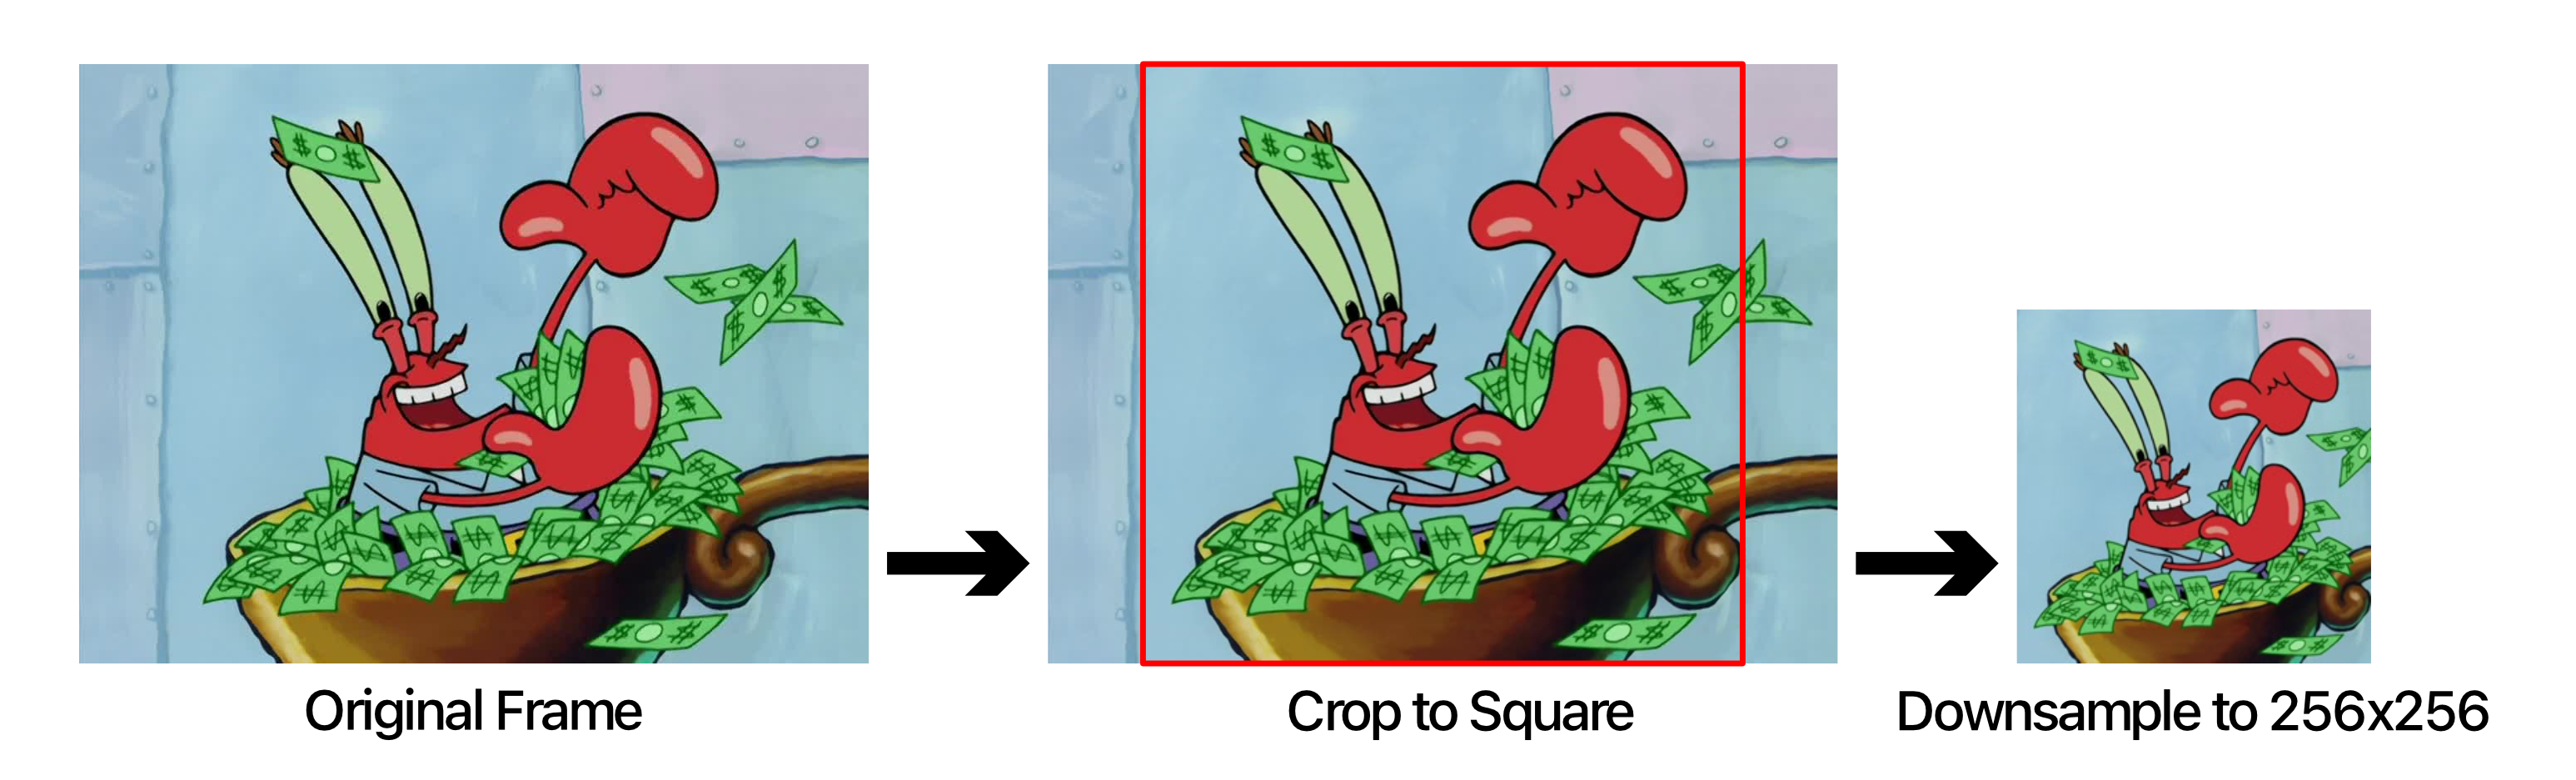
\includegraphics[width=\linewidth]{crop.png}
  \caption{ffmpeg cropping process}
  \label{fig:crop}
\end{figure}


The following is an example of the FFmpeg \cite{noauthor_ffmpeg_nodate} command used to obtain the raw images from the episodes:

\vskip 0.1in
 \begin{verbatim}
ffmpeg -i "season/episode.mkv"
-ss 63 -r 1/2 -s 256x256 -f image2
-vf "crop=720:720:114:0"
out/season/season-episode-\%03d.jpeg
\end{verbatim}

\subsubsection{Command Breakdown}
\verb|-i|- specifies the input file \newline
\verb|-ss 63 |- skips the first 63 seconds, or to the closet frame.\newline
\verb|-r 1/2 |- sets the rate of frames per second - 1/2 one frame every 2 seconds. \newline
\verb|-s 256x256 |- resizes the image to the given parameter - 256x256 in this case.\newline
\verb|-f image2  |- manually specifies output of the format jpeg.\newline
\verb|-vf "crop=720:720:114:0"|- crops the image to the given parameter, in this case it keeps the center square of the frame. \newline

}

\subsection{Model}
\label{sec:model}
{\quad
After proper data preparation and with enough training data, the model could now be built and trained. The initial build of the initial model consisted of four layers, an input layer, a convolution layer,a pooling layer, and a dense layer. This model yielded results more impressive than the first model's design, but through experimentation it was discovered that adding a few extra layers improved accuracy. The final model consists of seven layers by adding a second convolution layer, a second pooling layer, and a dropout layer to the previous model. The model is compiled using Keras' Adam optimizer as the optimizer parameter and sparse\_categorical\_crossentropy as the loss function. To further obtain the best results, hyper-parameters in the model (learning rate, boolean for dropout, etc) are tuned using KerasTuner - more on this in the following section \ref{sec:tuner}. Because of the limited data, a batch size of 16 was used when training the model and the validation split was 20\%. The following sample sizes were used for the training of the model:
\vskip 0.1in
\begin{center}
\begin{tabular}{||c | c||} 
 \hline
 Characters & Samples \\ [0.5ex] 
 \hline
 Spongebob & 245 \\ 
 \hline
 Patrick & 106 \\
 \hline
 Squidward & 114 \\
 \hline
 Mr Krabs & 89 \\ [1ex]
 \hline
\end{tabular}
\end{center}
}
\vskip 0.1in

\subsubsection{KerasTuner}
\label{sec:tuner}
% \lipsum[7]
{\quad
The KerasTuner \cite {omalley2019kerastuner} is a general-purpose hyperparameter tuning library that is extremely useful in providing the best values for hyperparameters to achieve the best results. For the SpongeDetect model, the defined search space consits of a float hyperparameter for the learning rate used within the compilation of the model and a boolean hyperparameter to determine whether or not to include the dropout layer in the model. The tuner class selected for this model that runs the search is Hyperband and its specified objective to optimize is the validation data's accuracy. Tuning the hyperparamters through a series of trials at ten epochs per trial yielded the following results for the highest scoring trial:
 \begin{verbatim}
Score: Validation accuracy = 0.945454537
Float: learning\_rate = 0.00049547586024
Boolean: dropout = False
 \end{verbatim}
}

\section{Results}

{\quad 
After preparing data, building the model, training the model, tuning the model, and testing and tweaking the model, the accuracy was finally satisfactory. To obtain final results for the model, more Spongebob images for each character were obtained from episodes of a season not previously used in the training or validation data. Approximately ten images of each character not yet seen by the model were used to test the models ability to predict. 

Predictions:

\begin{figure}[H]
  \begin{center}
    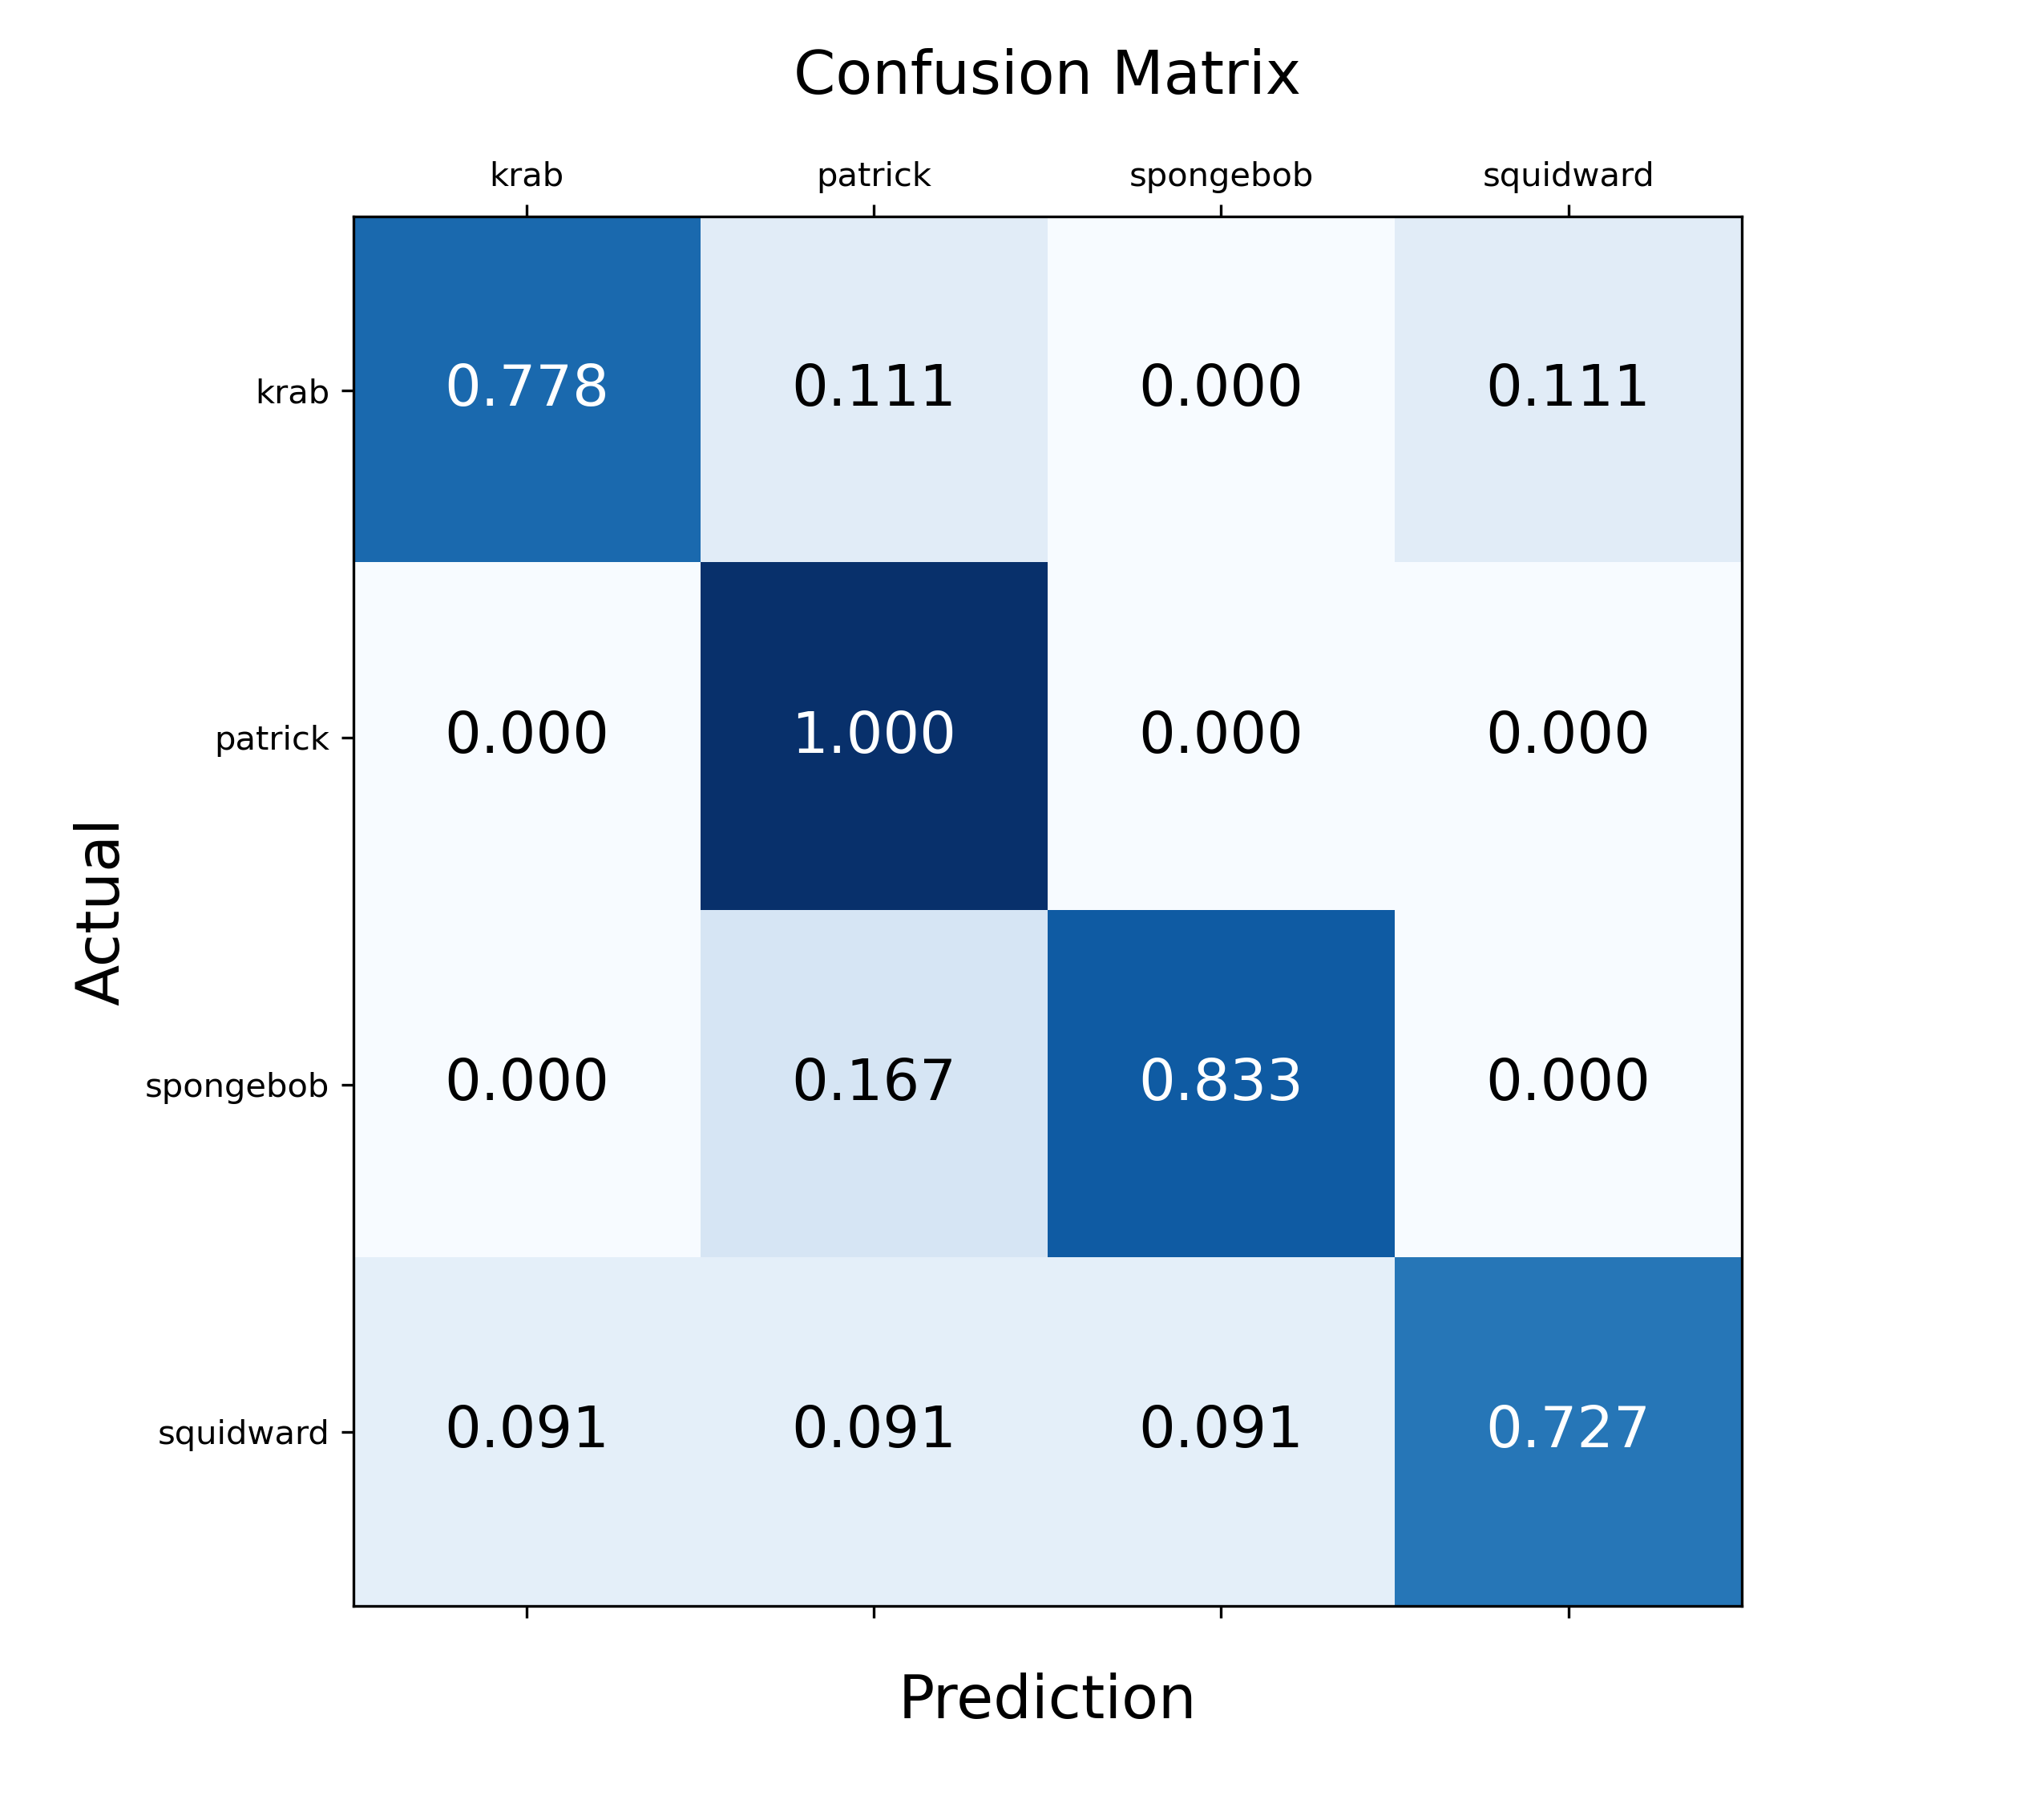
\includegraphics[width=\linewidth]{confusion_matrix.png}
  \end{center}
  \caption{A confusion matrix of predictions made on unseen data.}
  \label{fig:confusion}
\end{figure}

The confusion matrix shows impressive results in that the model can very accurately predict the characters based on the limited data the model was trained with. 

}
\section{Conclusion}
{\quad
In conclusion, TensorFlow and Keras are extremely useful tools for developing machine learning models, and with proper layering and tuning can yield extremely accurate results. Not only can the developed model accurately classify images of Spongebob characters, it can revolutionize the world in that no one can ever forget which character was which in the cartoon. Convolutional neural networks will change the way that society identifies Spongebob characters and can even be applied to subjects beyond the Spongebob realm. Soon enough people will not have a need to store the names of these characetrs in their minds, but can simply rely on the magic behind the learning machine. Spongebob shall forever remain on top thanks to the power of machine learning. 
}

\end{multicols}

%Bibliography
\bibliographystyle{IEEEtran}
\bibliography{references}  

\end{document}
